% Chapter "HHL" -- build with:  latexmk -pdf hhl_chapter.tex
% Companion of book/qft_chapter_source/qft_chapter.tex (same layout, box styles and section pattern).
% Figures are shared with the lecture: run presentations/hhl_source/make_figures.py first.
\documentclass[11pt,a4paper,openany]{book}
\usepackage[a4paper, top=22mm, bottom=22mm, left=22mm, right=22mm, headheight=14pt]{geometry}
\usepackage[T1]{fontenc}
\usepackage{lmodern}
\usepackage{amsmath, amssymb, mathtools, amsthm}
\usepackage{braket}
\usepackage{array, tabularx, booktabs}
\usepackage{enumitem}
\usepackage[dvipsnames]{xcolor}
\usepackage[most]{tcolorbox}
\usepackage{graphicx}
\usepackage{tikz}
\usetikzlibrary{quantikz2, arrows.meta, positioning}
\usepackage{fancyhdr}
\usepackage[hidelinks]{hyperref}
\usepackage{needspace}
\graphicspath{{../../presentations/hhl_source/figures/}}

\definecolor{brand}{HTML}{1F4E79}
\definecolor{okgreen}{HTML}{1B7F3B}
\definecolor{warn}{HTML}{B5551B}
\setlength{\parindent}{0pt}
\setlength{\parskip}{5pt}
\setlength{\emergencystretch}{3em}
\allowdisplaybreaks

\newtcolorbox{defn}[1]{enhanced, breakable, colback=brand!5, colframe=brand, fonttitle=\bfseries, title={Definition: #1}}
\newtcolorbox{keyres}[1]{enhanced, breakable, colback=okgreen!5, colframe=okgreen!70!black, fonttitle=\bfseries, title={Key result: #1}}
\newtcolorbox{trap}{enhanced, breakable, colback=warn!6, colframe=warn, fonttitle=\bfseries, title={Common trap}}
\newtcolorbox{method}[1]{enhanced, breakable, colback=black!3, colframe=black!55, fonttitle=\bfseries, title={Method: #1}}
\newtcolorbox{checklist}{enhanced, breakable, colback=white, colframe=black!35, fonttitle=\bfseries, title={Checklist}}
\newcounter{wex}[chapter]
\newtcolorbox{wexample}[1]{enhanced, breakable, colback=white, colframe=brand!60, coltitle=black, colbacktitle=brand!15,
  fonttitle=\bfseries, title={\refstepcounter{wex}Worked example \thesection.\arabic{wex}: #1}}
\newenvironment{steps}{\begin{enumerate}[label=\textbf{Step \arabic*.}, leftmargin=4.2em, itemsep=2pt]}{\end{enumerate}}

\pagestyle{fancy}\fancyhf{}
\fancyhead[L]{\small\color{black!70}Chapter: HHL}
\fancyhead[R]{\small\color{black!70}\rightmark}
\fancyfoot[C]{\small\thepage}
\renewcommand{\headrulewidth}{0.4pt}
\renewcommand{\thesection}{\arabic{section}}
\renewcommand{\sectionmark}[1]{\markright{\thesection.\ #1}}
\newcommand{\lt}{\tilde\lambda}

\begin{document}
\begin{titlepage}
\centering
{\color{brand}\rule{\linewidth}{1.5pt}}\\[10pt]
{\Huge\bfseries\color{brand} HHL}\\[8pt]
{\LARGE The Quantum Linear-Systems Algorithm}\\[6pt]
{\large A step-by-step chapter: from $Ax = b$ to a CUDA-Q implementation}\\[6pt]
{\color{brand}\rule{\linewidth}{1.5pt}}
\vspace{18mm}

\begin{minipage}{0.86\linewidth}
\large
\textbf{What you will be able to do after this chapter}
\begin{itemize}[itemsep=3pt]
\item solve small linear systems through the eigen-decomposition and compute condition numbers, sparsity and classical costs;
\item amplitude-encode vectors, evaluate $e^{iAt}$ and explain why HHL needs Hermitian, invertible, well-conditioned matrices;
\item run quantum phase estimation by hand, including inexact phases and two's-complement (negative) clock values;
\item derive every state of the HHL algorithm: eigenvalue inversion, the constant $C$, the ancilla, uncomputation and post-selection;
\item compute success probabilities, read-out statistics and the norm of $x$, and judge the complexity claims honestly;
\item read and modify \texttt{HHL.ipynb}, and interpret its circuit statistics and results;
\item solve every type of question in the accompanying 80-question HHL assessment.
\end{itemize}
\end{minipage}
\vfill
{\small Companion material in the same repository: \texttt{presentations/HHL\_Lecture.pdf} (slides),
\texttt{HHL.ipynb} (CUDA-Q notebook) and \texttt{assessments/} (question paper and answer book).}
\end{titlepage}

\tableofcontents
\setcounter{chapter}{0}
\chapter*{HHL --- The Quantum Linear-Systems Algorithm}
\addcontentsline{toc}{chapter}{HHL --- The Quantum Linear-Systems Algorithm}
\markboth{HHL}{HHL}

\section*{How to use this chapter}
The chapter is built as a staircase. Sections~1--2 are the \emph{linear algebra} you need (linear systems, eigen-decomposition, Hermitian
matrices, condition number, sparsity) and how vectors become \emph{quantum states}. Section~3 is the \emph{quantum toolkit} (controlled unitaries,
the QFT and phase estimation). Sections~4--5 are \emph{HHL itself}: the algorithm derived line by line and fully worked examples. Sections~6--7
cover \emph{what you can read out} and \emph{what it costs}. Sections~8--9 cover the \emph{implementation} in \texttt{HHL.ipynb}, its results,
noise, limitations and newer algorithms. Section~10 collects problem-solving strategies and maps every assessment question to the section
that teaches it; Section~11 has practice problems with answers.

Each section has: the idea in words, the precise statement, a derivation, \textbf{worked examples} solved step by step,
\textbf{common traps} (the wrong answers examiners like to offer) and a short checklist. Statements are marked as \emph{general
theory}, \emph{the notebook's implementation}, or \emph{illustrative examples}. ``Recorded'' results are the outputs stored in \texttt{HHL.ipynb};
``re-executed'' results were produced again with CUDA-Q~0.16 (\texttt{qpp-cpu}) from the notebook's circuit code. Every number was recomputed
with NumPy or CUDA-Q (\texttt{assessments/hhl\_test\_source/verify\_answers.py}, \texttt{presentations/hhl\_source/make\_figures.py}).

\begin{defn}{Conventions used everywhere in this chapter}
\begin{itemize}[leftmargin=1.2em, itemsep=1pt]
\item $A$ is $d\times d$ with $d = 2^{n_b}$; eigenpairs $A\ket{u_j} = \lambda_j\ket{u_j}$; $\ket b = \sum_j\beta_j\ket{u_j}$ with $\beta_j = \braket{u_j|b}$.
\item $U = e^{iAt}$ (the notebook's sign), $n_c$ clock qubits, $M = 2^{n_c}$, $C = 2\pi/(Mt)$. Clock value of $\lambda$: $k = \lambda t M/(2\pi) = \lambda/C$.
\item Clock register: \texttt{clock[0]} is the \textbf{most significant bit}; values $k \ge M/2$ are negative: $\tilde k = k - M$ (two's complement).
\item $R_Y(\theta) = e^{-i\theta Y/2}$, so $R_Y(\theta)\ket0 = \cos\frac\theta2\ket0 + \sin\frac\theta2\ket1$.
\item $\mathrm{QFT}\ket c = \frac{1}{\sqrt M}\sum_ke^{2\pi i\,ck/M}\ket k$.
\item The notebook's default system: $A = H\,\mathrm{diag}(1, 2, 3, 4)\,H$ with $H = \frac12\begin{psmallmatrix}1&1&1&1\\1&-1&1&-1\\1&1&-1&-1\\1&-1&-1&1\end{psmallmatrix}$,
      $b = (1, 0, 0, 0)$, $n_c = 4$, $t = \pi/8$, $C = 1$, 7 qubits, $20\,000$ shots, seed 42.
\end{itemize}
\end{defn}

%=====================================================================================================
\section{Linear systems and the linear algebra behind HHL}
\subsection{Linear systems}
A linear system $Ax = b$ has a unique solution $x = A^{-1}b$ exactly when $A$ is \textbf{invertible}: $\det A \ne 0$, equivalently no eigenvalue is $0$.
\begin{wexample}{a $2\times2$ system by elimination}
$A = \begin{psmallmatrix}1&-1/3\\-1/3&1\end{psmallmatrix}$, $b = (1, 0)$ (the notebook's $2\times2$ example).
\begin{steps}
\item $\det A = 1 - \frac19 = \frac89 \ne 0$.
\item $A^{-1} = \frac{1}{\det A}\begin{psmallmatrix}1&1/3\\1/3&1\end{psmallmatrix} = \frac98\begin{psmallmatrix}1&1/3\\1/3&1\end{psmallmatrix}$.
\item $x = A^{-1}b = \frac98(1, \tfrac13) = (\tfrac98, \tfrac38) = (1.125, 0.375)$. Check: $1.125 - 0.375/3 = 1$ and $-1.125/3 + 0.375 = 0$ \checkmark.
\end{steps}
\end{wexample}

\subsection{Hermitian matrices and the eigen-decomposition}
\begin{keyres}{spectral theorem}
A Hermitian matrix ($A = A^\dagger$; real symmetric if real) has real eigenvalues and an orthonormal eigenbasis:
$A = \sum_j\lambda_j\ket{u_j}\bra{u_j}$. If no $\lambda_j$ is $0$,
\[ A^{-1} = \sum_j\frac{1}{\lambda_j}\ket{u_j}\bra{u_j},\qquad A^{-1}\ket b = \sum_j\frac{\beta_j}{\lambda_j}\ket{u_j}. \]
\end{keyres}
Inverting $A$ means \emph{dividing each eigen-component of $b$ by its eigenvalue}. HHL does precisely this, for all components at once, in
superposition. Other classes: unitary matrices have $|\lambda| = 1$; positive-definite matrices have $\lambda > 0$; projectors have $\lambda\in\{0, 1\}$
(and are singular unless $P = I$).
\begin{wexample}{solving through the eigenbasis}
$A = \begin{psmallmatrix}2&1\\1&2\end{psmallmatrix}$, $b = (2, 1)$.
\begin{steps}
\item $\lambda_1 = 3$, $\ket{u_1} = \frac{1}{\sqrt2}(1, 1)$; $\lambda_2 = 1$, $\ket{u_2} = \frac{1}{\sqrt2}(1, -1)$.
\item $\beta_1 = \frac{2 + 1}{\sqrt2} = \frac{3}{\sqrt2}$, $\beta_2 = \frac{2 - 1}{\sqrt2} = \frac{1}{\sqrt2}$.
\item $x = \frac{3/\sqrt2}{3}\ket{u_1} + \frac{1/\sqrt2}{1}\ket{u_2} = \frac12(1, 1) + \frac12(1, -1) = (1, 0)$. Check: $A(1, 0) = (2, 1)$ \checkmark.
\end{steps}
\end{wexample}
\begin{wexample}{the notebook's default matrix}
$H$ is symmetric and orthogonal ($H^2 = I$), so $A = H\,\mathrm{diag}(1, 2, 3, 4)\,H$ has eigenvalues $1, 2, 3, 4$ and eigenvectors = the columns of $H$.
Writing it out,
\[ A = \begin{pmatrix} 2.5 & -0.5 & -1 & 0\\ -0.5 & 2.5 & 0 & -1\\ -1 & 0 & 2.5 & -0.5\\ 0 & -1 & -0.5 & 2.5\end{pmatrix}. \]
Check: trace $= 10 = 1 + 2 + 3 + 4$; each row has 3 non-zeros.
\end{wexample}

\subsection{Non-Hermitian matrices: the embedding}
Phase estimation reads eigenvalues of the \emph{unitary} $e^{iAt}$, which is unitary for every $t$ only if $A$ is Hermitian. A general $A$ is embedded:
\[ \tilde A = \begin{pmatrix}0 & A\\ A^\dagger & 0\end{pmatrix},\qquad \tilde A\begin{pmatrix}y\\ x\end{pmatrix} = \begin{pmatrix}b\\ 0\end{pmatrix}
\ \Longleftrightarrow\ Ax = b,\ A^\dagger y = 0\ (\Rightarrow y = 0). \]
The solution sits in the \textbf{second half}; the dimension doubles (one more system qubit). The eigenvalues of $\tilde A$ are $\pm\sigma_i$, the singular values
of $A$ with both signs --- so the embedded system always has \textbf{negative eigenvalues}. Dimensions that are not powers of 2 are padded with an identity block.
\begin{wexample}{embedding $\begin{psmallmatrix}1&2\\0&1\end{psmallmatrix}$ (notebook, Section 4 table)}
\begin{steps}
\item $A^\dagger A = \begin{psmallmatrix}1&2\\2&5\end{psmallmatrix}$ has eigenvalues $3 \pm 2\sqrt2$, so $\sigma = \sqrt2 \pm 1 = 2.4142, 0.4142$; $\kappa = (\sqrt2 + 1)^2 = 5.83$.
\item $\tilde A$ is $4\times4$ with eigenvalues $\pm2.4142$, $\pm0.4142$; $n_b = 2$, so with $n_c = 4$ the circuit has $4 + 2 + 1 = 7$ qubits.
\item $\kappa = 5.83 \le 7$: ``auto'' time maps $0.4142$ to clock value 1, $C = 0.4142$; then $2.4142$ maps to $5.83$ --- \emph{not an integer}.
\item Simulating the notebook's circuit (NumPy and CUDA-Q agree): $P_{\text{success}} = 0.1696$, recovered second half $(-1.0085, 0.9796)$ vs.\ the exact
      $x = (-1, 1)$, fidelity $0.99979$. The rounding of $5.83$ costs a little accuracy.
\end{steps}
\end{wexample}
\begin{trap}
``The embedded system's solution is the first half'' --- no: $(y, x)$ with $x$ in the second half. And ``padding with an identity block is harmless'' --- it adds
the eigenvalue $1$: a $3\times3$ matrix with eigenvalues $5, 10, 20$ ($\kappa = 4$) becomes $4\times4$ with $\kappa = 20/1 = 20$ for the clock.
\end{trap}

\subsection{The condition number}
\begin{defn}{condition number}
$\kappa(A) = \|A\|\,\|A^{-1}\| = \sigma_{\max}/\sigma_{\min} \ge 1$; for Hermitian $A$, $\kappa = |\lambda|_{\max}/|\lambda|_{\min}$. It is unchanged by $A \to cA$ ($c \ne 0$).
\end{defn}
$\kappa$ is the worst-case amplification of relative errors: $\frac{\|\delta x\|}{\|x\|} \le \kappa\,\frac{\|\delta b\|}{\|b\|}$.
\begin{wexample}{error amplification}
$A = \mathrm{diag}(1, 0.01)$ ($\kappa = 100$), $b = (1, 0)$, $x = (1, 0)$. Perturb $b$ by $\delta b = (0, 0.01)$ (relative size $0.01$): $\delta x = (0, 1)$ (relative size $1$).
The error grew by exactly $100 = \kappa$.
\end{wexample}
For HHL, $\kappa$ decides three things: how many clock qubits are needed to resolve $\lambda_{\min}$ next to $\lambda_{\max}$, how small the
success probability can be (Section~4.6), and therefore the run time (Section~7).
\begin{trap}
$\kappa$ is a ratio of eigenvalue \emph{magnitudes} --- not $\lambda_{\max} - \lambda_{\min}$, not $\lambda_{\max}/\lambda_{\min}$ with signs. Unitary matrices have $\kappa = 1$.
\end{trap}

\subsection{Sparsity and classical cost}
A matrix is \textbf{$s$-sparse} if every row has at most $s$ non-zero entries (the default $A$: $s = 3$). Sparse matrices need $O(ds)$ storage and
$O(ds)$ work per product $Av$.
\begin{center}\small
\begin{tabular}{lll}
\toprule method & cost & remark\\ \midrule
Gaussian elimination / LU & $\frac23d^3$ flops & dense; doubling $d$ costs $8\times$\\
Conjugate gradient (positive definite) & $O(d\,s\sqrt\kappa\log(1/\varepsilon))$ & iterations $\propto\sqrt\kappa$\\
CG on the normal equations (general $A$) & $O(d\,s\,\kappa\log(1/\varepsilon))$ & squares the condition number\\
HHL (Section~7) & $\tilde O(\log(d)\,s^2\kappa^2/\varepsilon)$ & returns $\ket x$, not $x$\\ \bottomrule
\end{tabular}
\end{center}
The notebook's reference solution is \texttt{np.linalg.solve} (LU). Any classical method that writes down $x$ costs at least $d$.
\begin{checklist}
Invertible? Hermitian (or embedded, solution in the second half)? $\kappa$ from eigenvalue \emph{magnitudes}? Did padding add the eigenvalue 1?
\end{checklist}

%=====================================================================================================
\section{From vectors to quantum states}
\subsection{Amplitude encoding}
\begin{defn}{amplitude encoding}
A vector $b\in\mathbb C^d$, $d = 2^{n}$, is stored in $n$ qubits as $\ket b = \frac{1}{\|b\|}\sum_ib_i\ket i$. Only the direction is stored; $\|b\|$ is kept classically.
\end{defn}
\begin{wexample}{encoding and measuring}
$b = (3, 0, 4, 0)$: $\|b\| = 5$, $\ket b = 0.6\ket{00} + 0.8\ket{10}$ (index $i = 2q_0 + q_1$). Measuring gives $\ket{00}$ with probability $0.36$ and $\ket{10}$ with $0.64$:
the first qubit is $\ket1$ with probability $0.64$, the second qubit is always $\ket0$.
\end{wexample}
Exponential compactness cuts both ways: $n$ qubits hold $2^n$ amplitudes, but a generic $\ket b$ needs $O(2^n)$ elementary gates to prepare (Möttönen,
Shende--Bullock--Markov), and reading the amplitudes back needs many measurements. Efficient preparation needs structure in $b$ or a QRAM.
\textbf{In the notebook}, the whole initial state $\ket0_c\ket b\ket0_a$ is loaded with \texttt{kernel.qalloc(vector)} --- a simulator feature without gates;
the reported gate counts do not include state preparation.

\subsection{Unitary time evolution $e^{iAt}$}
For Hermitian $A = \sum_j\lambda_j\ket{u_j}\bra{u_j}$: $e^{iAt} = \sum_je^{i\lambda_jt}\ket{u_j}\bra{u_j}$ --- same eigenvectors, eigenvalues on the unit circle,
unitary for every real $t$ (it is \emph{not} unitary in general if $A$ is not Hermitian).
\begin{wexample}{two exponentials}
\begin{steps}
\item $A = \mathrm{diag}(1, 2)$, $t = \pi/2$: $e^{iAt} = \mathrm{diag}(e^{i\pi/2}, e^{i\pi}) = \mathrm{diag}(i, -1)$.
\item $A = X$ (Pauli): $X^2 = I$, so $e^{iXt} = \cos t\,I + i\sin t\,X$. At $t = \pi/2$: $iX$.
\end{steps}
\end{wexample}
\textbf{Hamiltonian simulation} is the task of implementing $e^{iAt}$ with gates. For $A = \sum_kA_k$ with simple pieces, the Trotter product
$\big(\prod_ke^{iA_kt/r}\big)^r$ has error $O(t^2/r)$ (first order); sparse matrices are split into 1-sparse pieces; modern methods (qubitization, quantum signal
processing) are near-optimal. \textbf{In the notebook} there is no Hamiltonian simulation: \texttt{U\_step = expm(1j * A\_work * t\_evolution)} is the exact
matrix exponential, registered as a custom gate.

\subsection{Memory of a simulated state}
A state vector of $N$ qubits has $2^N$ complex amplitudes: $16\cdot2^N$ bytes in fp64, $8\cdot2^N$ in fp32; a density matrix needs $16\cdot4^N$.
The default HHL circuit ($N = 7$) needs $2048$ bytes; the notebook's memory line counts one extra copy for \texttt{get\_state} (about $4.1$ kB).
With $n_c = 8$ ($N = 11$): $32\,768$ bytes per copy. Memory is never the bottleneck of these small instances; gate count and depth are.
\begin{checklist}
Normalised amplitudes? Probabilities $= |\text{amplitude}|^2$? Gate cost of state preparation counted (or explicitly excluded)?
\end{checklist}

%=====================================================================================================
\section{Phase estimation: the engine of HHL}
\subsection{Controlled unitaries and phase kick-back}
A controlled-$V$ gate is $\ket0\bra0\otimes I + \ket1\bra1\otimes V$. If the target is an eigenvector, $V\ket u = e^{i\phi}\ket u$, then
\[ \tfrac{1}{\sqrt2}(\ket0 + \ket1)\ket u \longmapsto \tfrac{1}{\sqrt2}(\ket0 + e^{i\phi}\ket1)\ket u: \]
the phase is \textbf{kicked back} onto the control; the target is unchanged. A controlled-$U^{2^j}$ can be built as $2^j$ controlled-$U$ gates, or (cheaper) by
simulating $e^{iA\,t2^j}$ directly; the notebook registers $U^{2^j}$ = \texttt{matrix\_power(U, 2**j)} as one custom gate.

\subsection{The quantum Fourier transform}
$\mathrm{QFT}\ket c = \frac{1}{\sqrt M}\sum_{k}e^{2\pi i\,ck/M}\ket k$ is unitary, so $\mathrm{QFT}^{-1} = \mathrm{QFT}^\dagger$ (reverse the gate order and negate the angles).
Its inverse maps a \textbf{phase ramp} to a basis state:
\[ \mathrm{QFT}^{-1}:\ \frac{1}{\sqrt M}\sum_{c=0}^{M-1}e^{2\pi i\,ck/M}\ket c \longmapsto \ket k. \]
\textbf{Notebook implementation} ($n_c$ clock qubits): the inverse QFT is \texttt{swap}s first, then for $j = n_c - 1, \dots, 0$ the controlled phases
\texttt{cr1}$(-\pi/2^{k-j})$ on qubit $j$, controlled by each less significant qubit $k > j$, then \texttt{h} on qubit $j$. The QFT in the uncomputation is its exact mirror image
(\texttt{h} and \texttt{cr1}$(+\pi/2^{k-j})$, then the swaps). For $n_c = 4$: 4 \texttt{h}, 6 \texttt{cr1}, 2 \texttt{swap} each.
\begin{center}
\begin{quantikz}[row sep=0.3cm, column sep=0.3cm]
\lstick{$c_0$ (MSB)} & \swap{2} & & & & \gate{R_1(-\frac\pi4)} & \gate{R_1(-\frac\pi2)} & \gate{H} &\\
\lstick{$c_1$} & & & \gate{R_1(-\frac\pi2)} & \gate{H} & & \ctrl{-1} & &\\
\lstick{$c_2$} & \targX{} & \gate{H} & \ctrl{-1} & & \ctrl{-2} & & &
\end{quantikz}\\[1mm]
{\small The notebook's inverse QFT for $n_c = 3$, in code order.}
\end{center}

\subsection{Quantum phase estimation}
\begin{keyres}{phase estimation}
Let $U\ket u = e^{2\pi i\phi}\ket u$, $\phi\in[0, 1)$. With $n$ clock qubits, $M = 2^n$:
\begin{enumerate}[itemsep=1pt]
\item $H^{\otimes n}$: $\frac{1}{\sqrt M}\sum_c\ket c\ket u$;
\item controlled $U^{2^j}$ by the clock qubit of weight $2^j$ (together: $U^c$ on $\ket c$): $\frac{1}{\sqrt M}\sum_ce^{2\pi i\phi c}\ket c\ket u$;
\item $\mathrm{QFT}^{-1}$: if $M\phi = k$ is an integer, the result is exactly $\ket k\ket u$. Otherwise outcome $k$ has probability
      \[ P(k) = \Big|\frac1M\sum_{c=0}^{M-1}e^{2\pi ic(\phi - k/M)}\Big|^2, \]
      and the nearest integer to $M\phi$ has $P \ge 4/\pi^2 \approx 0.405$.
\end{enumerate}
\end{keyres}
\begin{center}
\begin{quantikz}[row sep=0.3cm, column sep=0.3cm]
\lstick{$\ket0$ \ $c_0$ (weight 4)} & \gate{H} & & & \ctrl{3} & \gate[3]{\mathrm{QFT}^{-1}} & \meter{}\\
\lstick{$\ket0$ \ $c_1$ (weight 2)} & \gate{H} & & \ctrl{2} & & & \meter{}\\
\lstick{$\ket0$ \ $c_2$ (weight 1)} & \gate{H} & \ctrl{1} & & & & \meter{}\\
\lstick{$\ket u$} & \qwbundle{n_b} & \gate{U} & \gate{U^2} & \gate{U^4} & &
\end{quantikz}
\end{center}
\begin{wexample}{exact and inexact phases with two clock qubits}
\begin{steps}
\item $\phi = \frac14$: after step 2 the clock holds $\frac12(\ket0 + i\ket1 - \ket2 - i\ket3)$ (phases $e^{2\pi ic/4} = 1, i, -1, -i$). This is $\mathrm{QFT}\ket1$, so
      $\mathrm{QFT}^{-1}$ gives $\ket{01}$ with probability 1: $\phi = 0.01_2$.
\item $\phi = \frac13 = 0.0101\ldots_2$: $P(k) = (0.0625, 0.6998, 0.1875, 0.0502)$ for $k = 0, 1, 2, 3$. The nearest $k = 1$ wins with $\approx0.70$; the rest \textbf{leaks}.
\item $\phi = \frac{3}{16}$ with four clock qubits: $16\phi = 3$, outcome $\ket{0011}$ with certainty.
\end{steps}
\end{wexample}

\subsection{Phase estimation with $U = e^{iAt}$: eigenvalues in the clock}
With $U = e^{iAt}$ the eigenphase of $\ket{u_j}$ is $\phi_j = \lambda_jt/(2\pi)$ and the clock reads
\[ k_j = M\phi_j = \frac{\lambda_j\,t\,2^{n_c}}{2\pi} = \frac{\lambda_j}{C},\qquad C = \frac{2\pi}{2^{n_c}t}. \]
One clock step is worth $C$ in eigenvalue units. Phases are taken modulo 1, so a \textbf{negative} eigenvalue $\lambda < 0$ appears as $k = M + \lambda/C$:
\begin{center}\small
\begin{tabular}{c|cccccccc}
register $k$ ($n_c = 3$) & 0 & 1 & 2 & 3 & 4 & 5 & 6 & 7\\ \hline
signed $\tilde k$ & 0 & 1 & 2 & 3 & $-4$ & $-3$ & $-2$ & $-1$
\end{tabular}
\end{center}
For $n_c = 4$: $3 = \texttt{0011}$, $8 \to -8$, $12 \to -4$, $15 \to -1$. Consequences: the representable signed range is $-M/2, \dots, M/2 - 1$, so we need $|\lambda|t < \pi$;
an eigenvalue beyond the range \textbf{aliases} (with $n_c = 4$, $t = \pi/8$: $\lambda = 9$ is read as $9 - 16 = -7$). Shifting $A \to A + I$ shifts every clock value by $1/C$.
\begin{wexample}{the default system}
$n_c = 4$, $t = \pi/8$: $k_j = \lambda_j\cdot\frac{(\pi/8)\cdot16}{2\pi} = \lambda_j$. With $\beta_j = \frac12$, after phase estimation
\[ \tfrac12\big(\ket{u_1}\ket{0001} + \ket{u_2}\ket{0010} + \ket{u_3}\ket{0011} + \ket{u_4}\ket{0100}\big)\ket0_a. \]
System and clock are now \textbf{entangled} (a product state only if $\ket b$ is a single eigenvector).
\end{wexample}
\begin{trap}
Measuring the clock now would collapse the superposition onto one eigenvector: it estimates \emph{one} eigenvalue, it does not solve the system. And
$k_j = \lambda_jt/(2\pi)$ is the phase, not the clock value --- multiply by $2^{n_c}$.
\end{trap}
\begin{checklist}
Which clock qubit is the MSB? Is $M\phi$ an integer? Negative eigenvalue $\Rightarrow$ $k - M$? Is $|\lambda|t < \pi$?
\end{checklist}

%=====================================================================================================
\section{The HHL algorithm, step by step}
\subsection{Registers}
\begin{center}\small
\begin{tabular}{llll}
\toprule register & qubits & role & default\\ \midrule
clock & $n_c$ & phase estimation: holds $\lambda_j/C$ in binary & 4 (qubits 0--3)\\
system & $n_b = \log_2d$ & starts in $\ket b$, ends in $\ket x$ & 2 (qubits 4--5)\\
ancilla & 1 & rotated by $C/\lt$; outcome 1 = success & 1 (qubit 6)\\ \midrule
total & $n_c + n_b + 1$ & & 7\\ \bottomrule
\end{tabular}
\end{center}
Example: an $8\times8$ Hermitian system with $n_c = 5$ needs $5 + 3 + 1 = 9$ qubits.

\subsection{The circuit}
\begin{center}
\resizebox{\linewidth}{!}{%
\begin{quantikz}[row sep=0.45cm, column sep=0.35cm]
\lstick{clock $\ket0^{\otimes n_c}$} & \qwbundle{n_c} & \gate{H^{\otimes n_c}} & \ctrl{1} & \gate{\mathrm{QFT}^{-1}} & \ctrl{2} & \gate{\mathrm{QFT}} & \ctrl{1} & \gate{H^{\otimes n_c}} & \meter{} & \rstick{$=0$}\\
\lstick{system $\ket b$} & \qwbundle{n_b} & & \gate{U^c} & & & & \gate{U^{-c}} & & \meter{} & \rstick{$\sim|x_i|^2$}\\
\lstick{ancilla $\ket0$} & & & & & \gate{R_Y(\theta_k)} & & & & \meter{} & \rstick{$=1$}
\end{quantikz}}
\end{center}
``Controlled $U^c$'' denotes the $n_c$ gates $U^{2^j}$, each controlled by one clock qubit; the inversion block is a set of rotations controlled on the
clock value $k$.

\subsection{The state after every stage}
\begin{keyres}{HHL state evolution (exact clock values)}
\begin{align*}
&\text{0. initial} && \ket0_c\ket b\ket0_a = \textstyle\sum_j\beta_j\ket0_c\ket{u_j}\ket0_a\\
&\text{1--2. phase estimation} && \textstyle\sum_j\beta_j\ket{k_j}\ket{u_j}\ket0_a\\
&\text{3. eigenvalue inversion} && \textstyle\sum_j\beta_j\ket{k_j}\ket{u_j}\Big(\sqrt{1 - \frac{C^2}{\lambda_j^2}}\ket0 + \frac{C}{\lambda_j}\ket1\Big)\\
&\text{4. uncomputation} && \textstyle\sum_j\beta_j\ket0_c\ket{u_j}\Big(\sqrt{1 - \frac{C^2}{\lambda_j^2}}\ket0 + \frac{C}{\lambda_j}\ket1\Big)\\
&\text{5. ancilla} = 1 && \dfrac{C\sum_j\frac{\beta_j}{\lambda_j}\ket{u_j}}{\sqrt{P_{\text{success}}}} = \ket x,\qquad P_{\text{success}} = C^2\sum_j\frac{|\beta_j|^2}{\lambda_j^2} = C^2\,\|A^{-1}\ket b\|^2.
\end{align*}
\end{keyres}
\emph{Derivation of step 5.} The ancilla-$\ket1$ part of step 4 is $\ket0_c\otimes C\sum_j\frac{\beta_j}{\lambda_j}\ket{u_j}\otimes\ket1 = \ket0_c\otimes C\,A^{-1}\ket b\otimes\ket1$
(Section 1.2). Its squared norm is the probability of measuring 1; dividing by its norm gives $\ket x$.

\subsection{Eigenvalue inversion and the constant $C$}
The rotation $R_Y(\theta)\ket0 = \cos\frac\theta2\ket0 + \sin\frac\theta2\ket1$ with
\[ \theta_k = 2\arcsin\frac{C}{\lt_k},\qquad \lt_k = C\,\tilde k, \]
puts amplitude $C/\lt_k$ on $\ket1$ --- this is how a unitary ``divides by $\lambda$''. Requirements and consequences:
\begin{itemize}[itemsep=2pt]
\item $|C/\lt| \le 1$ for every eigenvalue: $C \le |\lambda|_{\min}$. The largest allowed $C$ maximises $P_{\text{success}}$, so the best choice is $C = |\lambda|_{\min}$.
\item Negative $\lt$ gives a negative angle: the sign of $1/\lambda$ is kept in the amplitude.
\item In the notebook $C = 2\pi/(2^{n_c}t)$ is the eigenvalue of clock value 1 (the smallest representable $|\lt|$), and the rotation for register $k$ is
      $\theta = 2\arcsin(1/\tilde k)$; with the ``auto'' time and $\kappa \le 2^{n_c-1} - 1$ this means $C = |\lambda|_{\min}$.
\end{itemize}
\begin{wexample}{rotation angles of the default run}
$C = 1$, $\lt = 1, 2, 3, 4$: $\sin\frac\theta2 = 1, \frac12, \frac13, \frac14$, i.e.\ $\theta = \pi$, $\frac\pi3 = 1.0472$, $2\arcsin\frac13 = 0.6797$, $2\arcsin\frac14 = 0.5054$ rad.
The ancilla-$\ket1$ probabilities for single eigenvectors are $1, \frac14, \frac19, \frac1{16}$. Register $12$ means $\tilde k = -4$: amplitude $-\frac14$.
\end{wexample}
\textbf{The notebook's lookup table.} For every register value $k = 1, \dots, 2^{n_c} - 1$ (zero is skipped --- no eigenvalue 0): apply \texttt{x} to every clock
qubit that is 0 in $k$ (``polarity'' gates, so that the control fires only on $\ket k$), apply $R_Y(\theta_k)$ controlled on \emph{all} $n_c$ clock qubits
(\texttt{kernel.cry(theta, clock, ancilla)}, recorded as \texttt{ccccry} for $n_c = 4$), undo the \texttt{x} gates. That is $2^{n_c} - 1$ rotations
(15 for $n_c = 4$, 255 for $n_c = 8$) --- exponential in $n_c$. Scalable designs compute $1/\lt$ with reversible arithmetic or approximate $1/x$ by a
polynomial (QSVT, Section~9).
\begin{figure}[h]
\centering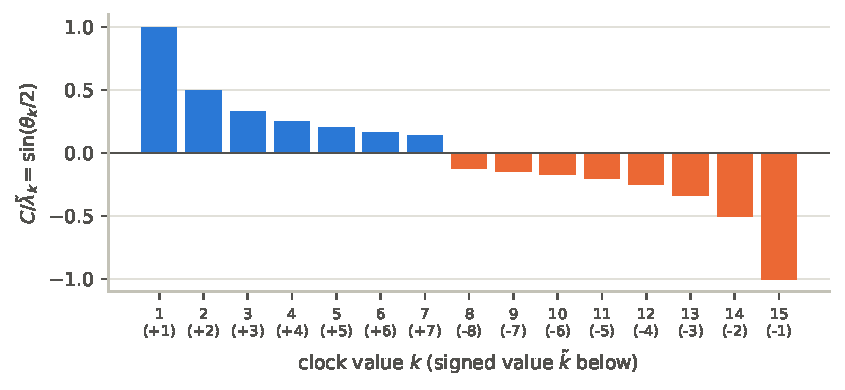
\includegraphics[width=0.78\linewidth]{inversion_table}
\caption{Ancilla amplitude $C/\lt_k$ for the 15 non-zero clock values of the default run ($n_c = 4$, $C = 1$); register values $\ge8$ are negative.}
\end{figure}

\subsection{The ancilla and uncomputation}
$A^{-1}$ is not unitary, so it cannot be a gate. HHL embeds it as one block of a larger unitary on system + ancilla: the $\ket1$ branch carries
$C\,A^{-1}\ket b$, the $\ket0$ branch the rest. The price is a \textbf{probabilistic} outcome.

Before uncomputation the clock is entangled with the system. Post-selecting the ancilla at that point would leave the system \textbf{mixed}:
the branches $\ket{k_j}$ are orthogonal, so the terms $\frac{\beta_j}{\lambda_j}\ket{u_j}$ cannot interfere into $\ket x$. Inverse phase estimation
(QFT, controlled $U^{-2^j}$ = \texttt{matrix\_power(U.conj().T, 2**j)}, $H^{\otimes n_c}$) returns every $\ket{k_j}$ to $\ket0$ and disentangles the clock.
If some $k_j$ were not integers, the clock would not return exactly to $\ket0$; the notebook therefore keeps only shots with clock $= 0$ \emph{and} ancilla $= 1$.

\subsection{Success probability and repetitions}
\begin{keyres}{success probability bounds}
With $C = |\lambda|_{\min}$: $\ \dfrac{1}{\kappa^2} \le P_{\text{success}} = \sum_j|\beta_j|^2\dfrac{C^2}{\lambda_j^2} \le 1$.
Lower bound: all weight on $|\lambda|_{\max}$. Upper bound: all weight on $|\lambda|_{\min}$.
\end{keyres}
Repeat-until-success needs $1/P_{\text{success}}$ runs on average; \textbf{amplitude amplification} needs $O(1/\sqrt{P_{\text{success}}})$ (e.g.\ $P = 0.01$: about 100 vs.\ about 10).
In the worst case this turns $\kappa^2$ repetitions into $\kappa$.
\begin{figure}[h]
\centering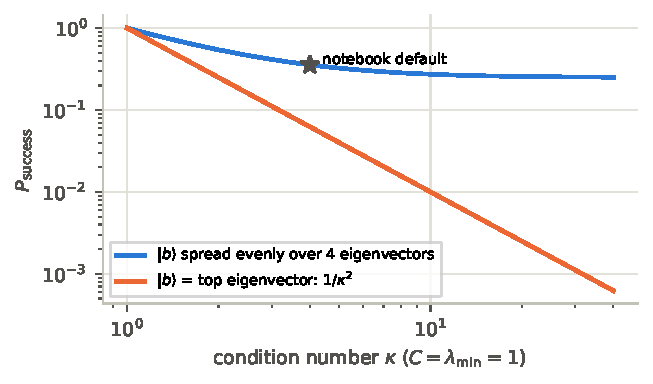
\includegraphics[width=0.62\linewidth]{kappa_success}
\caption{Illustrative: $P_{\text{success}}$ versus $\kappa$ ($C = \lambda_{\min} = 1$) for $\ket b$ spread evenly over four eigenvectors with evenly spaced eigenvalues
in $[1, \kappa]$, and for $\ket b$ equal to the top eigenvector ($1/\kappa^2$). The star is the notebook's default, $0.3559$.}
\end{figure}
\begin{trap}
$C/\lambda$ is an \emph{amplitude}; the probability is $C^2/\lambda^2$. $P_{\text{success}}$ is \emph{not} $C\|A^{-1}b\|$, and it does not depend on $\kappa$ alone but on where $b$ lives.
\end{trap}
\begin{checklist}
$C \le |\lambda|_{\min}$? Angles $\theta = 2\arcsin(C/\lt)$ (factor 2!)? Sign of negative eigenvalues kept? Clock uncomputed before reading the system?
\end{checklist}

%=====================================================================================================
\section{Fully worked problems}
\begin{wexample}{the notebook's $2\times2$ example}
$A = \begin{psmallmatrix}1&-1/3\\-1/3&1\end{psmallmatrix}$, $b = (1, 0)$, $n_c = 4$, ``auto'' time.
\begin{steps}
\item $\lambda_1 = \frac23$, $\ket{u_1} = \frac{1}{\sqrt2}(1, 1)$; $\lambda_2 = \frac43$, $\ket{u_2} = \frac{1}{\sqrt2}(1, -1)$; $\kappa = 2 \le 7$.
\item $t = \frac{2\pi}{16\cdot\frac23} = \frac{3\pi}{16}$, $C = \lambda_{\min} = \frac23$; clock values $k = \lambda/C = 1, 2$ (exact).
\item $\beta_1 = \beta_2 = \frac{1}{\sqrt2}$; rotation amplitudes $C/\lambda = 1, \frac12$.
\item Ancilla-1 branch: $\frac{1}{\sqrt2}\cdot1\cdot\ket{u_1} + \frac{1}{\sqrt2}\cdot\frac12\ket{u_2} = \frac12(1, 1) + \frac14(1, -1) = (\frac34, \frac14)$.
\item $P_{\text{success}} = \frac9{16} + \frac1{16} = \frac58 = 0.625$; $\ket x = \frac{1}{\sqrt{10}}(3, 1)$; sampled frequencies $0.9$ and $0.1$.
\item Norm recovery: $x = \frac{\|b\|}{C}(\frac34, \frac14) = \frac32(\frac34, \frac14) = (1.125, 0.375)$ \checkmark. Re-executed with CUDA-Q: $P = 0.625000$, fidelity $1.0000000000$.
\end{steps}
\end{wexample}

\begin{wexample}{the notebook's default $4\times4$ system}
\begin{steps}
\item $\beta_j = \braket{u_j|b} = H_{0j} = \frac12$ for all four eigenvectors; $t = \pi/8$, $C = 1$, $k_j = \lambda_j = 1, 2, 3, 4$.
\item Ancilla-1 branch: $\sum_j\frac12\cdot\frac{1}{\lambda_j}\ket{u_j} = H\cdot\frac12(1, \frac12, \frac13, \frac14)$:
      \[ x = \tfrac14\big(1 + \tfrac12 + \tfrac13 + \tfrac14,\ 1 - \tfrac12 + \tfrac13 - \tfrac14,\ 1 + \tfrac12 - \tfrac13 - \tfrac14,\ 1 - \tfrac12 - \tfrac13 + \tfrac14\big)
         = \tfrac{1}{48}(25, 7, 11, 5). \]
\item Decimals: $(0.520833, 0.145833, 0.229167, 0.104167)$ --- equal to \texttt{np.linalg.solve}. Because $C = \|b\| = 1$, the amplitudes \emph{are} $x$.
\item $P_{\text{success}} = \|x\|^2 = \frac{625 + 49 + 121 + 25}{2304} = \frac{820}{2304} = \frac{205}{576} = 0.355903$, also $= \frac14(1 + \frac14 + \frac19 + \frac1{16})$.
      $\|x\| = \sqrt{0.355903} = 0.5966$.
\item Shot probabilities: \[ |x_i|^2/\|x\|^2 = (625, 49, 121, 25)/820 = (0.7622,\ 0.0598,\ 0.1476,\ 0.0305). \]
\item With $20\,000$ shots, about $0.355903\times20\,000 \approx 7118$ are accepted (recorded: 7086).
\end{steps}
\end{wexample}

\begin{wexample}{a diagonal system with three clock qubits}
$A = \mathrm{diag}(1, 2)$, $\ket b = \frac{1}{\sqrt2}(1, 1)$, $n_c = 3$, $t = \pi/4$.
\begin{steps}
\item $C = \frac{2\pi}{8\cdot\pi/4} = 1$; clock values $k = \lambda$: $1 = \texttt{001}$ and $2 = \texttt{010}$.
\item After phase estimation: $\frac{1}{\sqrt2}(\ket0\ket{001} + \ket1\ket{010})$ (system $\otimes$ clock).
\item Ancilla-1 branch: $\frac{1}{\sqrt2}(1\cdot\ket0 + \frac12\ket1)$; $P_{\text{success}} = \frac12(1 + \frac14) = \frac58 = 0.625$.
\item $\ket x \propto (1, \frac12)$, normalised $\frac{1}{\sqrt5}(2, 1)$ --- matches $A^{-1}b \propto (1, \frac12)$.
\end{steps}
\end{wexample}

\begin{wexample}{a negative eigenvalue}
$A = \mathrm{diag}(1, -2)$, $\ket b = \frac{1}{\sqrt2}(1, 1)$, $n_c = 3$: $\kappa = 2 \le 3$, so $t = \frac{2\pi}{8\cdot1} = \frac\pi4$, $C = 1$.
\begin{steps}
\item Clock values: $\lambda = 1 \to 1$; $\lambda = -2 \to -2 \to 8 - 2 = 6 = \texttt{110}$.
\item The lookup table reads register 6 as $\tilde k = -2$: amplitude $C/\lt = -\frac12$ (negative angle).
\item Ancilla-1 branch: $\frac{1}{\sqrt2}(1, -\frac12)$, $P_{\text{success}} = 0.625$; $A^{-1}b = \frac{1}{\sqrt2}(1, -\frac12)$ \checkmark (sign preserved).
\end{steps}
\end{wexample}

\begin{wexample}{too few clock qubits (re-executed variant)}
Default system with $n_c = 3$: $k_{\max} = 3 < \kappa = 4$, so ``auto'' maps $\lambda_{\max} = 4$ to $3$: $t = \frac{2\pi\cdot3}{8\cdot4} = \frac{3\pi}{16}$, $C = \frac43$.
\begin{steps}
\item Clock values $\lambda\cdot\frac34 = 0.75, 1.5, 2.25, 3$: only $\lambda = 4$ is exact; the others leak over neighbouring registers (clock distribution: $P(1) = P(2) = 0.3147$, $P(3) = 0.2891$).
\item Re-executed with CUDA-Q: fidelity $0.9532157640$, $P_{\text{success}} = 0.3285$ from the state.
\item The notebook's printed ``ideal'' value $\sum_j|\beta_j|^2C^2/\lambda_j^2 = 0.632716$ uses $C/\lambda_1 = \frac43 > 1$ --- not a probability. The formula is valid only when
      $C \le |\lambda|_{\min}$ (here it is not); the circuit itself clips nothing, because every register value has $|\tilde k| \ge 1$.
\end{steps}
\end{wexample}
\begin{figure}[h]
\centering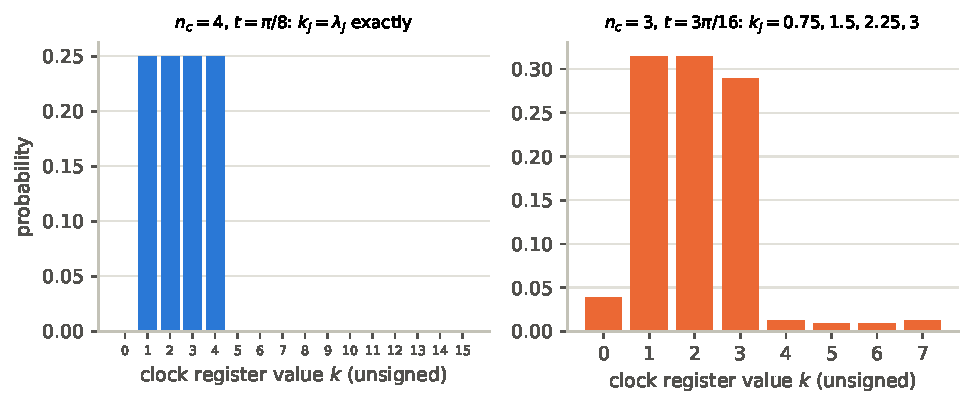
\includegraphics[width=0.9\linewidth]{clock_distribution}
\caption{Clock register after phase estimation for the default system (CUDA-Q, notebook circuit stopped after the inverse QFT). Left: $n_c = 4$, four exact
peaks of $\frac14$. Right: $n_c = 3$, rounded clock values spread over neighbouring registers.}
\end{figure}

%=====================================================================================================
\section{Reading out the solution}
\begin{keyres}{what $\ket x$ gives you}
\begin{itemize}[itemsep=1pt]
\item \textbf{Samples}: outcome $i$ with probability $|x_i|^2/\|x\|^2$ (magnitudes only).
\item \textbf{Expectation values} $\braket{x|M|x}$ of an observable $M$ --- the intended use.
\item \textbf{Overlaps} with another state via a swap test: $P(0) = \frac12\big(1 + |\braket{x|\phi}|^2\big)$.
\item \textbf{The norm}: $\|x\| = \frac{\|b\|}{C}\sqrt{P_{\text{success}}}$, so the success rate estimates $\|A^{-1}b\|$.
\end{itemize}
Estimating all $d$ components to precision $\varepsilon$ costs about $d/\varepsilon^2$ shots --- linear in $d$, no speed-up.
\end{keyres}
\begin{wexample}{statistics of the recorded run}
\begin{steps}
\item Accepted fraction: $7086/20\,000 = 0.3543$; its binomial standard error $\sqrt{p(1 - p)/S} = \sqrt{0.3559\cdot0.6441/20\,000} = 0.0034$. The deviation $0.0016$ is about half a standard error.
\item Component 0: sampled $0.7691$ vs.\ exact $0.7622$ (difference $0.0069$); standard error $\sqrt{0.7622\cdot0.2378/7086} = 0.0051$, so $1.4$ standard errors --- ordinary
      shot noise. The notebook quotes the conservative scale $1/\sqrt{7086} = 0.012$.
\item Norm from the success rate ($C = \|b\| = 1$): $\|x\| \approx \sqrt{0.3543} = 0.595$ (exact $0.5966$).
\item An expectation value: $Z$ on the first system qubit (the most significant bit) gives $\braket{Z\otimes I} = \frac{625 + 49 - 121 - 25}{820} = 0.6439$.
\end{steps}
\end{wexample}
\textbf{Signs and phases} are invisible in computational-basis samples: $x = (1, -1)$ and $(1, 1)$ give the same histogram. They need measurements in other
bases or interference with a reference state. \textbf{In the notebook} the simulator reads the amplitudes directly (\texttt{cudaq.get\_state}), takes the branch
clock $= 0$, ancilla $= 1$, and multiplies by $\|b\|/C$ --- full amplitude access that hardware does not provide.
\begin{figure}[h]
\centering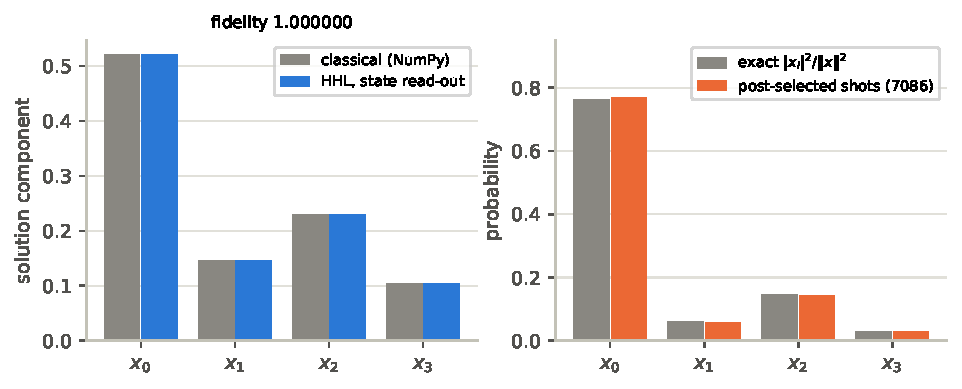
\includegraphics[width=0.95\linewidth]{default_solution}
\caption{Default run, re-executed with the notebook's circuit and seed 42 (identical to the recorded output). Left: state read-out vs.\ NumPy. Right: the 7086 post-selected shots
vs.\ the exact $|x_i|^2/\|x\|^2$.}
\end{figure}
\begin{trap}
``HHL outputs the vector $x$ exponentially faster'' --- it outputs a \emph{state}. Printing $x$ needs $O(d/\varepsilon^2)$ repetitions. And ``the norm is lost'' is also wrong:
the success probability carries $\|A^{-1}b\|$.
\end{trap}

%=====================================================================================================
\section{Complexity and its fine print}
\begin{keyres}{HHL running time (Harrow, Hassidim, Lloyd 2009)}
$\tilde O\big(\log(d)\,s^2\kappa^2/\varepsilon\big)$ for an $s$-sparse $d\times d$ matrix, condition number $\kappa$ and precision $\varepsilon$.
$\log d$: amplitude encoding and sparse Hamiltonian simulation; one $\kappa$ from the phase-estimation precision needed to resolve $\lambda_{\min}$,
one from the success probability (after amplitude amplification); $1/\varepsilon$ from phase estimation.
\end{keyres}
Compared with conjugate gradient ($O(d\,s\sqrt\kappa\log(1/\varepsilon))$ for positive-definite $A$), HHL is exponentially better in $d$ but worse in $\kappa$ and $\varepsilon$.
The speed-up survives only under all of the following (Aaronson, ``Read the fine print'', Nature Physics 2015):
\begin{enumerate}[itemsep=1pt]
\item $\ket b$ can be prepared in $\mathrm{polylog}(d)$ time;
\item $e^{iAt}$ can be applied efficiently ($A$ sparse or structured, accessed through an oracle);
\item $\kappa$ (and $1/\varepsilon$) grow at most polylogarithmically in $d$;
\item only a global property of $x$ is needed (an expectation value, an overlap, a norm).
\end{enumerate}
\textbf{Evidence on both sides.} HHL is BQP-complete: simulating all its instances classically would simulate any quantum computation, so in general no classical
algorithm matches it. On the other hand, ``dequantised'' algorithms (Tang 2018 and later) show that for \emph{low-rank} matrices with classical sampling access,
classical algorithms match the quantum scaling up to polynomial factors --- some proposed quantum advantages disappear.
\begin{wexample}{counting clock qubits for a given $\kappa$}
The notebook needs $\kappa \le 2^{n_c-1} - 1$ for exact clock values with ``auto'' time: $\kappa = 3 \to n_c = 3$; $\kappa = 7 \to 4$; $\kappa = 20 \to 6$ ($2^5 - 1 = 31 \ge 20$, while $2^4 - 1 = 15 < 20$);
$\kappa = 40 \to 7$. The circuit then has $2^{n_c} - 1$ rotations: $7, 15, 63, 127$.
\end{wexample}
\begin{wexample}{the worst-case success probability}
$\kappa = 20$, $C = \lambda_{\min}$, $\ket b$ = eigenvector of $\lambda_{\max}$: $P_{\text{success}} = (\lambda_{\min}/\lambda_{\max})^2 = 1/400 = 0.0025$, i.e.\ 400 repetitions on average
(about 20 with amplitude amplification).
\end{wexample}
\begin{trap}
``HHL gives an exponential speed-up for every linear system'' --- false: dense $A$, large $\kappa$, expensive $\ket b$ or needing all of $x$ each remove it.
\end{trap}

%=====================================================================================================
\section{The implementation in \texttt{HHL.ipynb}}
\subsection{Structure and parameters}
\begin{enumerate}[itemsep=1pt]
\item Section 3 (inputs): \texttt{MATRIX\_A = "example"} (or \texttt{"random"} or a list), \texttt{VECTOR\_B = "example"}, \texttt{RANDOM\_SIZE = 4},
\texttt{RANDOM\_CONDITION\_NUMBER = 4.0}, \texttt{NUM\_CLOCK\_QUBITS = 4}, \texttt{EVOLUTION\_TIME = "auto"}, \texttt{BACKEND = "auto"},
\texttt{SIMULATION\_METHOD = "statevector"} (allowed: \texttt{"statevector"}, \texttt{"density\_matrix"}), \texttt{SHOTS = 20000}, \texttt{SEED = 42}.
\item Section 4: build and validate (square $A$, matching $b$, $b \ne 0$, $|\det A| \ge 10^{-12}$ and $\mathrm{cond}(A) \le 10^{12}$), \texttt{x\_classical = np.linalg.solve(...)},
Hermitian embedding, identity padding, eigenvalues, $\kappa$, $n_c \ge 2$, the time $t$, $C$ and the qubit count.
\item Section 6: expected results \emph{before} running: $\ket x$, the ``ideal'' $P_{\text{success}}$, whether the mapping is exact, memory, a gate estimate.
\item Section 7: \texttt{build\_hhl\_kernel} with the kernel builder (\texttt{cudaq.make\_kernel}), drawing, \texttt{cudaq.estimate\_resources} statistics.
\item Section 8: \texttt{cudaq.get\_state} (amplitude read-out) and \texttt{cudaq.sample} (shots), with live memory monitoring.
\item Sections 9--10: tables, plots, benchmark report in \texttt{exports/hhl/}.
\end{enumerate}
\begin{keyres}{the ``auto'' evolution time}
With $k_{\max} = 2^{n_c-1} - 1$: if $\kappa \le k_{\max}$, $t = \dfrac{2\pi}{2^{n_c}|\lambda|_{\min}}$ ($|\lambda|_{\min}\to$ clock value 1, $C = |\lambda|_{\min}$);
otherwise $t = \dfrac{2\pi k_{\max}}{2^{n_c}|\lambda|_{\max}}$ ($|\lambda|_{\max}\to k_{\max}$; small eigenvalues are rounded and $C > |\lambda|_{\min}$).
\end{keyres}

\subsection{The circuit code}
The builder allocates one register initialised with $\ket0_c\otimes\ket b\otimes\ket0_a$ (bit-reversed, because CUDA-Q's state vector treats qubit 0 as the
least significant bit), then:
\begin{enumerate}[itemsep=1pt]
\item \texttt{h} on every clock qubit; for $j = 0, \dots, n_c - 1$ a custom gate \texttt{matrix\_power(U, 2**j)} called as \texttt{kernel.<name>(clock[n\_c-1-j], *system)}
      (first argument = control; \texttt{clock[0]} is the MSB);
\item inverse QFT (\texttt{swap}, \texttt{cr1}$(-\pi/2^{k-j})$, \texttt{h});
\item for $k = 1, \dots, 2^{n_c} - 1$: \texttt{signed = k - 2**nc if k >= 2**(nc-1) else k}, \texttt{theta = 2*arcsin(clip(C/lam\_k, -1, 1))}, polarity \texttt{x} gates,
      \texttt{kernel.cry(theta, clock, ancilla)}, polarity \texttt{x} gates;
\item QFT, \texttt{swap}s, \texttt{matrix\_power(U.conj().T, 2**j)}, \texttt{h};
\item optionally \texttt{mz(reg)}: the bitstring is clock $|$ system $|$ ancilla, qubit 0 first.
\end{enumerate}
Read-out: \texttt{postselected\_amplitudes} reshapes the state into $2\times\cdots\times2$, reverses the axes and takes index $(0,\dots,0, :, \dots, :, 1)$;
\texttt{x\_quantum = amplitudes * b\_norm / C\_constant}, then the embedding/padding slice. Shots are kept if \texttt{bits[:n\_c] == "0"*n\_c} and \texttt{bits[-1] == "1"}.
With \texttt{"density\_matrix"} the dominant eigenvector of $\rho$ is used and its arbitrary global phase is aligned with NumPy's solution (a density matrix carries no global phase).
Hardware backends are refused with a \texttt{ValueError}: exact matrix exponentials as custom gates and amplitude loading cannot run on a QPU.

\subsection{Circuit size}
Counting the builder's gates for $n_c$ clock qubits ($n_b = 2$):
\[ \underbrace{4n_c}_{\texttt{h}} + \underbrace{2n_c}_{\text{custom}} + \underbrace{2\lfloor n_c/2\rfloor}_{\texttt{swap}} + \underbrace{n_c(n_c - 1)}_{\texttt{cr1}}
   + \underbrace{2\big(n_c2^{n_c-1} - n_c\big)}_{\texttt{x}} + \underbrace{2^{n_c} - 1}_{\text{rotations}}. \]
(The \texttt{x} count: register values $1, \dots, 2^{n_c} - 1$ contain $n_c2^{n_c-1} - n_c$ zero bits in total, each flipped twice.)
\begin{center}\small
\begin{tabular}{cccccc}
\toprule $n_c$ & qubits & gates & rotations & depth & multi-qubit\\ \midrule
2 & 5 & 23 & 3 & 21 & 11\\
3 & 6 & 51 & 7 & 38 & 21\\
4 & 7 & 111 & 15 & 67 & 39\\
5 & 8 & 235 & 31 & 120 & 65\\
6 & 9 & 507 & 63 & 221 & 111\\
7 & 10 & 1099 & 127 & 418 & 189\\ \bottomrule
\end{tabular}
\end{center}
{\small From \texttt{cudaq.estimate\_resources} on the notebook's builder (4$\times$4 system, ``auto'' time, measurements and the amplitude loading not counted).}
The recorded default ($n_c = 4$): \texttt{h} 16, custom 8, \texttt{swap} 4, \texttt{cr1} 12, \texttt{x} 56, \texttt{ccccry} 15 $= 111$ gates; 39 multi-qubit; depth 67.
The notebook's pre-run estimate of ``$\sim$107 gates'' uses a simpler formula (it counts $1 + n_c$ gates per rotation instead of the actual \texttt{x} gates) --- an estimate, not a count.

\subsection{Results}
\begin{center}\small
\begin{tabular}{llcccc}
\toprule run & settings & $C$ & $P_{\text{success}}$ (state) & fidelity & accepted shots\\ \midrule
recorded & default, $n_c = 4$ & 1 & 0.355903 & 1.0000000000 & 7086 / 20000\\
re-executed & default, $n_c = 4$ & 1 & 0.355903 & 1.0000000000 & 7086 / 20000\\
re-executed variant & default, $n_c = 3$ & $\frac43$ & 0.3285 & 0.9532157640 & ---\\
re-executed variant & default, $n_c = 2$ & 4 & 0.4222 & 0.2059 & ---\\
re-executed variant & $2\times2$ example & $\frac23$ & 0.625000 & 1.0000000000 & ---\\ \bottomrule
\end{tabular}
\end{center}
Relative error of the recovered $x$: $1.655\times10^{-15}$ (recorded), $1.74\times10^{-15}$ (re-executed) --- floating-point level. Recorded timings on a CPU (\texttt{qpp-cpu}):
construction $0.0056$ s, compilation $0.0524$ s, state run $0.0018$ s, sampling run $0.0758$ s. No GPU timing was measured for this material.
\begin{figure}[h]
\centering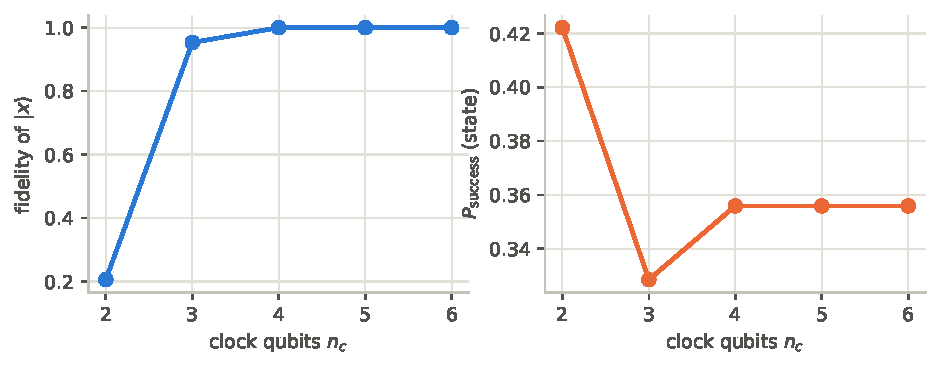
\includegraphics[width=0.8\linewidth]{precision}
\caption{Fidelity and success probability of the default system versus $n_c$ (``auto'' time, CUDA-Q state read-out, re-executed). From $n_c = 4$ every clock value is an integer.}
\end{figure}
\begin{trap}
A high $P_{\text{success}}$ is not a good result: at $n_c = 2$ it is $0.42$ while the fidelity is $0.21$. Always check the fidelity (or the relative error) as well.
\end{trap}
\begin{checklist}
Recorded, re-executed or illustrative number? Which $t$ and $C$ did ``auto'' pick? Embedded/padded system sliced back? Hardware claims --- none.
\end{checklist}

%=====================================================================================================
\section{Noise, limitations and advanced algorithms}
\subsection{Errors}
\textbf{Algorithmic} (present without noise): phase-estimation rounding when $k_j \notin \mathbb Z$ (Section 5), Hamiltonian-simulation error (absent in the notebook:
exact \texttt{expm}), finite shots ($\sim1/\sqrt{\text{accepted}}$). \textbf{Hardware noise} (general statements; not simulated in the notebook, which defines
no noise model even with \texttt{"density\_matrix"}): the multi-controlled rotations and controlled $e^{iAt2^j}$ decompose into many two-qubit gates; errors
in the clock spoil the uncomputation, and post-selection then accepts wrong shots. Practical HHL needs fault-tolerant hardware.

\subsection{Limitations}
General: state preparation of a generic $\ket b$ costs $O(d)$; $e^{iAt}$ must be efficient; the cost grows like $\kappa^2$ (or $\kappa$); the output is a state;
the circuits are deep. Notebook-specific: exact \texttt{expm} gates, amplitude loading by \texttt{qalloc(vector)}, a lookup-table inversion with $2^{n_c} - 1$ rotations,
full-matrix storage (sparsity not used), and simulator-only amplitude read-out.

\subsection{Applications and newer algorithms}
Proposed applications: discretised differential equations, least squares and other machine-learning kernels, electromagnetic scattering, network
quantities such as effective resistances --- always for a \emph{global property} of $x$, and none with a demonstrated end-to-end advantage.
\begin{center}\small
\begin{tabularx}{\linewidth}{@{}>{\raggedright\arraybackslash}p{5.2cm}>{\raggedright\arraybackslash}X@{}}
\toprule algorithm & key idea\\ \midrule
HHL (2009) & phase estimation + eigenvalue-controlled rotation; $\tilde O(\log(d)s^2\kappa^2/\varepsilon)$\\
Ambainis (2012) & variable-time amplitude amplification: $\kappa^2 \to \kappa$ (up to logarithms)\\
Childs--Kothari--Somma (2017) & linear combination of unitaries (Fourier/Chebyshev series of $1/x$) instead of phase estimation: $\mathrm{poly}\log(1/\varepsilon)$\\
QSVT (Gilyén et al.\ 2019) & polynomial approximation of $1/x$ applied to a block-encoding; unifies the above\\
Adiabatic and randomised methods (Suba\c{s}\i--Somma--Orsucci 2019), discrete adiabatic (Costa et al.\ 2022) & optimal $O(\kappa\log(1/\varepsilon))$ query complexity\\
Variational (VQLS) & short circuits and a classical optimiser; heuristic, no guarantee\\ \bottomrule
\end{tabularx}
\end{center}
None of these is implemented in \texttt{HHL.ipynb}; all share HHL's input and output caveats.

%=====================================================================================================
\section{Problem-solving strategies and question map}
\subsection{Strategy by question format}
\begin{itemize}[itemsep=3pt]
\item \textbf{Single-correct numerical:} compute fully, then sanity-check: $P_{\text{success}}\in[1/\kappa^2, 1]$; $|C/\lt| \le 1$; probabilities are squared amplitudes;
      clock values are $\lambda/C$, signed for $k \ge 2^{n_c-1}$. Typical distractors: ``amplitude instead of probability'', ``$\theta$ without the factor 2'',
      ``phase instead of clock value'', ``first half of the embedded solution'', ``forgot the square root'' (norm from $P$).
\item \textbf{Matching lists:} solve the easiest row first (often a definition or a one-line computation), then eliminate.
\item \textbf{Assertion--Reason:} judge A and R \emph{independently}; only if both are true ask whether R \emph{explains} A.
\item \textbf{Statement I/II:} one counterexample kills a ``for every'' statement; read code statements against the actual code (Section 8).
\item \textbf{Paragraph:} the first question sets up a quantity (eigenvalues, $\beta_j$, the state after QPE) reused in the second.
\end{itemize}
\subsection{Fast checks that catch most mistakes}
\begin{enumerate}[itemsep=2pt]
\item Verify a candidate solution by multiplying: $Ax = b$?
\item With $C = 1$ and $\|b\| = 1$: $P_{\text{success}} = \|x\|^2$.
\item Clock value $= \lambda t2^{n_c}/(2\pi)$; integer $\Rightarrow$ exact, otherwise leakage and fidelity $< 1$.
\item Gate counts: rotations $2^{n_c} - 1$; qubits $n_c + n_b + 1$; state vector $16\cdot2^N$ bytes.
\item Recorded vs.\ re-executed vs.\ illustrative --- which one does the question use?
\end{enumerate}
\subsection{Map: assessment questions $\to$ sections of this chapter}
\begin{tabularx}{\linewidth}{@{}>{\raggedright\arraybackslash}p{5.6cm}>{\raggedright\arraybackslash}X@{}}
\toprule
\textbf{Questions} & \textbf{Where to learn it}\\ \midrule
Q.1--Q.4, Q.7, Q.8, Q.19, Q.20 & Section 1 (systems, eigen-decomposition, matrix classes, condition number)\\
Q.6, Q.66, Q.67 & Section 1.3 and Section 8 (embedding and padding)\\
Q.9--Q.11 & Section 1.5 (sparsity, classical cost)\\
Q.12, Q.15--Q.17, Q.33, Q.34, Q.76 & Section 2 (encoding, $e^{iAt}$, memory)\\
Q.21--Q.26, Q.29, Q.30, Q.37--Q.40, Q.71 & Section 3 (controlled unitaries, QFT, phase estimation, signed clock values, aliasing)\\
Q.27, Q.28, Q.31, Q.32, Q.35, Q.41--Q.44, Q.48, Q.50--Q.52 & Section 4 (registers, inversion, $C$, ancilla, uncomputation)\\
Q.5, Q.13, Q.14, Q.18, Q.45, Q.53, Q.59, Q.60 & Section 5 (worked $2\times2$ and $4\times4$ problems)\\
Q.36, Q.54--Q.56, Q.62, Q.63, Q.79, Q.80 & Section 6 (read-out, shots, norm, swap test)\\
Q.61, Q.64, Q.68--Q.70, Q.78 & Section 7 (complexity, fine print, dequantisation)\\
Q.46, Q.47, Q.49, Q.57, Q.58, Q.65, Q.73--Q.75, Q.77 & Section 8 (the notebook: auto time, code, statistics, results)\\
Q.72 & Section 9 (advanced algorithms)\\
\bottomrule
\end{tabularx}
{\small (Section numbers: 1 linear algebra, 2 encoding, 3 phase estimation, 4 HHL algorithm, 5 worked problems, 6 read-out, 7 complexity,
8 notebook, 9 noise, limitations and advanced algorithms.)}

%=====================================================================================================
\section{Practice problems}
Try each before looking at the answers on the next page. They use the same ideas as the assessment but different numbers.
\begin{enumerate}[label=\textbf{P\arabic*.}, leftmargin=2.6em, itemsep=3pt]
\item Condition number of $\mathrm{diag}(4, 0.5)$.
\item Solve $\begin{psmallmatrix}3&1\\1&3\end{psmallmatrix}x = (4, 4)$ through the eigen-decomposition.
\item Amplitude-encode $b = (2, 0, 1, 2)$: $\ket b$ and the probability of $\ket{11}$.
\item $e^{iAt}$ for $A = \mathrm{diag}(1, 3)$ and $t = \pi/2$.
\item Phase estimation with 3 clock qubits on an eigenstate with $\phi = \frac38$: outcome and probability.
\item With $n_c = 3$, which signed value does register 5 represent?
\item $n_c = 5$ and $C = 0.5$: the clock value of $\lambda = 3$.
\item $C = 0.5$, $\lambda = 2$: rotation angle and probability of ancilla $= 1$ for that eigenvector.
\item $A = \mathrm{diag}(1, 4)$, $\ket b = \frac{1}{\sqrt2}(1, 1)$, $C = 1$: $P_{\text{success}}$ and $\ket x$.
\item $A = \mathrm{diag}(2, -1)$, $n_c = 3$, ``auto'' time: $t$, $C$ and the two register values.
\item A run succeeds with probability $0.04$. Expected repetitions with and without amplitude amplification.
\item Qubits and rotations of the notebook's circuit for a $16\times16$ Hermitian system with $n_c = 6$.
\item Use the gate-count formula of Section 8.3 for $n_c = 3$.
\item Standard error of the accepted fraction for $p = 0.25$ and $S = 10\,000$ shots.
\item $C = 1$, $\|b\| = 2$, measured success fraction $0.09$: estimate $\|x\|$.
\item A run prints an ``ideal'' $P_{\text{success}} = 0.63$ while the state gives $0.33$ and the fidelity is $0.95$. What happened?
\end{enumerate}

\newpage
\subsection*{Answers to the practice problems}
\begin{enumerate}[label=\textbf{P\arabic*.}, leftmargin=2.6em, itemsep=3pt]
\item $4/0.5 = 8$.
\item $b = (4, 4) = 4\sqrt2\,\ket{u_1}$ with $\lambda_1 = 4$, $\ket{u_1} = \frac{1}{\sqrt2}(1, 1)$: $x = \frac{4\sqrt2}{4}\ket{u_1} = (1, 1)$. Check: $A(1, 1) = (4, 4)$.
\item $\|b\| = 3$: $\ket b = \frac13(2\ket{00} + \ket{10} + 2\ket{11})$; $P(\ket{11}) = \frac49$.
\item $\mathrm{diag}(e^{i\pi/2}, e^{3i\pi/2}) = \mathrm{diag}(i, -i)$.
\item $8\phi = 3$: $\ket{011}$ with probability 1.
\item $5 - 8 = -3$.
\item $k = \lambda/C = 6$ (\texttt{00110}).
\item $\theta = 2\arcsin\frac{0.5}{2} = 2\arcsin\frac14 = 0.5054$ rad; $P = \frac1{16} = 0.0625$.
\item $P = \frac12(1 + \frac1{16}) = \frac{17}{32} = 0.53125$; $\ket x \propto (1, \frac14)$, i.e.\ $\frac{1}{\sqrt{17}}(4, 1)$.
\item $\kappa = 2 \le 3$: $t = \frac{2\pi}{8\cdot1} = \frac\pi4$, $C = 1$; $\lambda = 2 \to 2$ (\texttt{010}), $\lambda = -1 \to 8 - 1 = 7$ (\texttt{111}).
\item $1/0.04 = 25$ without; about $1/\sqrt{0.04} = 5$ with amplitude amplification.
\item $6 + 4 + 1 = 11$ qubits; $2^6 - 1 = 63$ rotations.
\item $12 + 6 + 2 + 6 + 2(12 - 3) + 7 = 51$ (matches \texttt{estimate\_resources}).
\item $\sqrt{0.25\cdot0.75/10\,000} = 0.0043$.
\item $\|x\| = \frac{\|b\|}{C}\sqrt P = 2\times0.3 = 0.6$.
\item $\kappa$ exceeded $2^{n_c-1} - 1$, so ``auto'' set $C > |\lambda|_{\min}$: the ``ideal'' formula used $C/\lambda > 1$ and is not a probability, and the eigenvalues were rounded
      (fidelity $< 1$). Increase \texttt{NUM\_CLOCK\_QUBITS} (this is exactly the $n_c = 3$ case of the default system).
\end{enumerate}

\subsection*{Summary of the chapter in ten lines}
\begin{enumerate}[itemsep=1pt]
\item $A^{-1}\ket b = \sum_j\frac{\beta_j}{\lambda_j}\ket{u_j}$: inversion is division in the eigenbasis of a Hermitian (or embedded) $A$.
\item $\kappa = |\lambda|_{\max}/|\lambda|_{\min}$ sets clock size, success probability and cost; padding can enlarge it.
\item Amplitude encoding stores a direction in $\log_2d$ qubits; preparing and reading it are the expensive ends.
\item Phase estimation with $U = e^{iAt}$ writes $k_j = \lambda_j/C$, $C = 2\pi/(2^{n_c}t)$; negative values in two's complement; non-integers leak.
\item $R_Y(2\arcsin(C/\lt))$ puts $C/\lambda_j$ on the ancilla; $C \le |\lambda|_{\min}$.
\item Uncompute the clock, post-select ancilla $= 1$: $\ket x$ with $P_{\text{success}} = C^2\|A^{-1}\ket b\|^2 \in [1/\kappa^2, 1]$.
\item Read-out: samples, expectation values, overlaps and the norm --- not the full vector ($d/\varepsilon^2$ shots).
\item Cost $\tilde O(\log(d)s^2\kappa^2/\varepsilon)$, valid only under the input/output fine print; newer algorithms reach $O(\kappa\log(1/\varepsilon))$.
\item \texttt{HHL.ipynb}: exact \texttt{expm} gates, lookup-table inversion, 7 qubits, 111 gates; $x = (25, 7, 11, 5)/48$ with fidelity 1 and $P = 0.3559$ --- reproduced with CUDA-Q.
\item Report honestly: recorded vs.\ re-executed vs.\ illustrative; check fidelity, not only $P_{\text{success}}$; no hardware or GPU claims without measurements.
\end{enumerate}
\end{document}
